\documentclass[
    UTF8,       % 编码格式
    b5paper,    % 纸张大小, I like b5
    10pt,       % 字号
    oneside,    % 书页排版 「 twoside, oneside 」
    openright,  % 新章节开始位置 「 openright, openany 」
    titlepage,  % 是否单独生成标题页
    final       % 草稿还是终稿 「 draft, final 」
]{ctexbook}
% 这里是导言区, 可以设置格式

% 数学公式
\usepackage{amsmath}
% \usepackage{arevmath}
% \usepackage[noend]{algpseudocode}
% \usepackage{algorithm}

% 算法样例
% \begin{algorithm}
% \caption{Put your caption here}
% \begin{algorithmic}[1]
% \Procedure{Roy}{$a,b$}                  \Comment{This is a test}
%     \State System Initialization
%     \State Read the value 
%     \If{$condition = True$}
%         \State Do this
%         \If{$Condition \geq 1$}
%         \State Do that
%         \ElsIf{$Condition \neq 5$}
%         \State Do another
%         \State Do that as well
%         \Else
%         \State Do otherwise
%         \EndIf
%     \EndIf
%     \While{$something \not= 0$}         \Comment{put some comments here}
%         \State $var1 \leftarrow var2$   \Comment{another comment}
%         \State $var3 \leftarrow var4$
%     \EndWhile  \label{roy's loop}
% \EndProcedure
% \end{algorithmic}
% \end{algorithm}

% 多列
%\usepackage{multicols}

% \usepackage{placeins} %\FloatBarrier要的包

% 页边距
\usepackage{geometry}
%\geometry{left=2cm,right=2cm,top=2cm,bottom=2cm}

% 页眉页脚
\usepackage{titlesec}
\usepackage{layout}
% \newpagestyle{article_style} { %
%     \headrule % 添加页眉处分割线
%     \footrule % 添加页脚处分割线
%     \setheadrule{10mm} % 注意在声明后设置长度才有效(也可以不设置长度)
%     \setfootrule{0.4pt} % 0.4pt 是分割线的默认值
%     \sethead
%     [第\thesection{}章 ~~\sectiontitle][][\thepage] %
%     {第\thesection{}章 ~~\sectiontitle}{}{\thepage}
%     \setfoot
%     [][\LaTeX{}游戏引擎开发笔记][]
%     {}{\LaTeX{}游戏引擎开发笔记}{}
% }

%\usepackage[printwatermark]{xwatermark}
% 水印
% \newwatermark[page=1,color=gray!20,angle=45,scale=4,xpos=0,ypos=0]
%     {Zhang Yf}
% \newwatermark[pages=2-4,color=gray!20,angle=45,scale=3,xpos=0,ypos=0]
%     {游戏引擎开发笔记}
% \newwatermark[pagex={5,6,7},color=gray!20,angle=45,scale=3,xpos=0,ypos=0]
%     {游戏引擎开发笔记}

% 下划线,斜体强调
\usepackage{ulem}
% \uline{}
% \emph{}

% 行距
\usepackage{setspace}
% \onehalfspacing

% 代码排版
\usepackage{listingsutf8}
% \usepackage{listings}
\usepackage{xcolor}
\usepackage{fontspec}
\usepackage{color}

\definecolor{dkgreen}{rgb}{0,0.6,0}
\definecolor{gray}{rgb}{0.5,0.5,0.5}
\definecolor{mauve}{rgb}{0.58,0,0.82}

% \lstset{
%     basicstyle          =   \sffamily,          % 基本代码风格
%     keywordstyle        =   \bfseries,          % 关键字风格
%     commentstyle        =   \rmfamily\itshape,  % 注释的风格,斜体
%     stringstyle         =   \ttfamily,  % 字符串风格
%     flexiblecolumns,                % 别问为什么,加上这个
%     numbers             =   left,   % 行号的位置在左边
%     showspaces          =   false,  % 是否显示空格,显示了有点乱,所以不现实了
%     numberstyle         =   \zihao{-5}\ttfamily,    % 行号的样式,小五号,tt等宽字体
%     showstringspaces    =   false,
%     captionpos          =   t,      % 这段代码的名字所呈现的位置,t指的是top上面
%     frame               =   lrtb,   % 显示边框
% }

\lstset{ %
    backgroundcolor =   \color{white},    % choose the background color
    basicstyle      =   \footnotesize\ttfamily, % size of fonts used for the code
    columns         =   fullflexible,
    tabsize         =   4,
    breaklines      =   true,             % automatic line breaking only at whitespace
    captionpos      =   b,                % sets the caption-position to bottom
    commentstyle    =   \color{mygreen},  % comment style
    escapeinside    =   {\%*}{*)},        % if you want to add LaTeX within your code
    keywordstyle    =   \color{blue},     % keyword style
    stringstyle     =   \color{mymauve}\ttfamily, % string literal style
    frame           =   single,
    rulesepcolor    =   \color{red!20!green!20!blue!20},
    identifierstyle =   \color{red},
    language        =   c++,
}

\lstdefinestyle{myPython}{
	frame               =   l,
	language            =   Python,
	aboveskip           =   3mm,
	belowskip           =   3mm,
	showstringspaces    =   false,
	columns             =   flexible,
	numberstyle         =   \small\color{red},
	basicstyle          =   {\small\ttfamily},
	keywordstyle        =   \color{blue},
	commentstyle        =   \color{dkgreen},
	stringstyle         =   \color{mauve},
	breaklines          =   true,
	breakatwhitespace   =   true,
    columns             =   fixed,
	tabsize             =   3,
    numbers             =   left,
}

\lstdefinestyle{C++}{
    language        =   C, % 语言选C
    basicstyle      =   \zihao{-5}\ttfamily,
    numberstyle     =   \zihao{-5}\ttfamily,
    keywordstyle    =   \bfseries\color{green!40!black},
	commentstyle    =   \itshape\color{purple!40!black},
	identifierstyle =   \color{blue},
	stringstyle     =   \color{orange},
    xleftmargin     =   \parindent,
    belowcaptionskip=   1\baselineskip,
    breaklines      =   true,   % 自动换行,建议不要写太长的行
    columns         =   fixed,  % 如果不加这一句,字间距就不固定,很丑,必须加
    basewidth       =   0.5em,
    numbers         =   left,
}

\lstdefinestyle{Lua}{
    language        =   C, % 语言选C++
    basicstyle      =   \zihao{-5}\ttfamily,
    numberstyle     =   \zihao{-5}\ttfamily,
    keywordstyle    =   \bfseries\color{green!40!black},
	commentstyle    =   \itshape\color{purple!40!black},
	identifierstyle =   \color{blue},
	stringstyle     =   \color{orange},
    xleftmargin     =   \parindent,
    belowcaptionskip=   1\baselineskip,
    breaklines      =   true,   % 自动换行,建议不要写太长的行
    columns         =   fixed,  % 如果不加这一句,字间距就不固定,很丑,必须加
    basewidth       =   0.5em,
    numbers         =   left,
}

% \lstinputlisting[
%     style       =   C,
%     caption     =   {\bf ff.py},
%     label       =   {ff.py}
% ]{../ff.py}

\makeatletter
\newenvironment{breakablealgorithm} 
    {% \begin{breakablealgorithm}
    \begin{center}
        \refstepcounter{algorithm}% New algorithm
        \hrule height.8pt depth0pt \kern2pt% \@fs@pre for \@fs@ruled
        \renewcommand{\caption}[2][\relax]{% Make a new \caption
        {\raggedright\textbf{\ALG@name~\thealgorithm} ##2\par}%
            \ifx\relax##1\relax % #1 is \relax
                \addcontentsline{loa}{algorithm}{\protect\numberline{\thealgorithm}##2}%
            \else % #1 is not \relax
                \addcontentsline{loa}{algorithm}{\protect\numberline{\thealgorithm}##1}%
            \fi
            \kern2pt\hrule\kern2pt
        }
    }{% \end{breakablealgorithm}
        \kern2pt\hrule\relax% \@fs@post for \@fs@ruled
    \end{center}
    }
\makeatother


\geometry{left=2.0cm,right=2.0cm,top=2.5cm,bottom=2.5cm}
\hypersetup{hidelinks}

% 标题作者
\title{3D引擎开发笔记}
\author{Zhang Yufeng \thanks{Email: 759094438@qq.com}}
\date{\today}

\begin{document}
    \maketitle
    \tableofcontents

    \frontmatter

    \maketitle
    \part{序言}

    \maketitle
    \chapter{序言}
    \section{新的开始}

从本科时期开始接触代码后,我便一直希望能够进行自己的项目开发,日常也喜欢写一些个人小程序自娱自乐,
因为一直对游戏较为感兴趣,因此初期希望研究并开发类似Unity的游戏引擎。
当然Unity是一个庞然大物,仅靠一个人是无法完成开发的,但是把目标放到Unity的部分功能来,这个计划就可行的多。
困于本科时期知识基础的薄弱,以及相关开发经验的缺乏,四年间都只做过一些较小的个人项目,
我的知识尚未形成一个较为完整的体系,也没有将个人的思想融入到项目中实现。

研究生阶段,为了在读研生涯中做点什么,希望留下自己的印记,我开始了这个项目的设计。
但是由于毕业与工作的压力,之前的文章写了部分就暂时搁浅了,而现在终于有时间来继续推进。
我的目标是将此项目作为一个小的完整的系统,搜集资料后按照个人的想法进行设计和实现,
不仅能够锻炼提升个人水平,还能够锻炼阅读写作与其他能力。
同时,这个系列的文章不仅是我个人学习过程的笔记,也将作为后续编写类似程序的相关参考,
并在这之中提出一些我个人的想法来抛砖引玉,得到他人的指导或同好的学习与分享。
最后希望通过此项目对其他做类似学习与开发的人做出一些微薄的贡献。

在这之中,感谢我的亲人、我的对象、我的老师与朋友对我的支持与帮助。

本文使用\LaTeX{} \footnote{\nolinkurl{https://mirrors.tuna.tsinghua.edu.cn/CTAN/info/lshort/chinese/lshort-zh-cn.pdf}} 编写,
使用\XeLaTeX{} 编译。

\maketitle
\section{初步的写作计划}

此项目聚焦于跨平台3D引擎的设计开发,从零开始搭建一个3D引擎用于渲染3D场景,
以及支持脚本及AI的场景内物体互动,使其具有成为仿真环境的可能性。
本项目模仿游戏引擎进行模块划分,一个游戏引擎由许多模块组成,
每个模块具有相对独立的功能,参考《游戏引擎架构》的内容,本文章将按照以下几个部分设计介绍。
当然也有部分章节可能脱离主线,介绍一些额外的内容。

本笔记主要参考的内容出自大名鼎鼎的Game Engine Architecture\footnote{\nolinkurl{https://www.gameenginebook.com/index.html}}的引擎架构,
该图附于本章最后。

这个原版的图片中的模块与功能过于完整与强大,有很多是我没有必要、也没有办法去实现的部分。经过简化后,我的引擎架构如下图所示:

\begin{figure}[H]
\centering
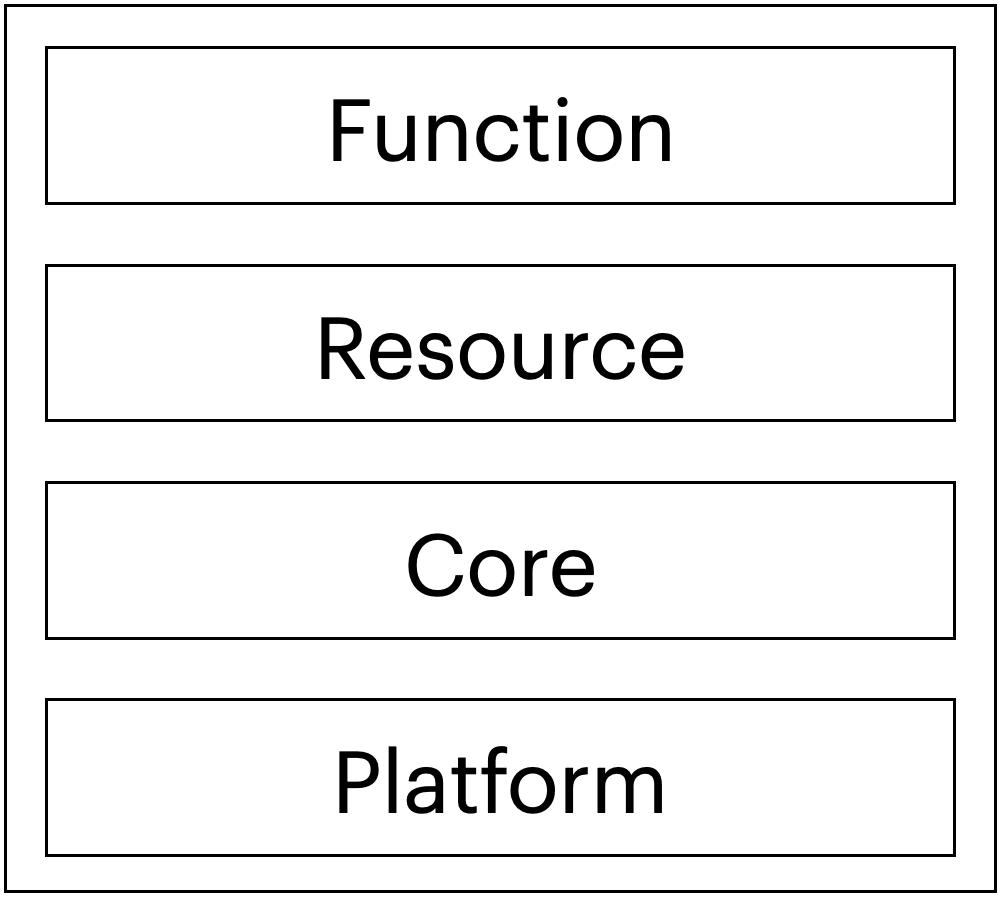
\includegraphics[center, width=0.30\textwidth]{chapter-front/pic/architecture.png}
\caption{简化的引擎架构图}
\end{figure}

该框架主要分为平台层、核心层、资源层、功能层与编辑器层。之后的各个章节将会按照分层的结构来组织。

\maketitle
\subsection{基础系统}

这个部分用于介绍引擎底层系统的设计,作为学习的必要过程,本项目中将跟随开发进度不断修改引擎底层结构的设计。许多基础的数据结构与算法也会出现在本节。

\maketitle
\subsection{数学与几何}

随后的渲染与物理部分,都与数学紧密相关。数学构成了渲染与物理模块的基石。本节主要介绍一些基本的数学内容,作为后续部分的基础。

\maketitle
\subsection{渲染系统}

为了能够展示场景的运行效果,需要有直观的方式展现内容,3D渲染就是最好的方式。这个部分主要介绍渲染的相关内容,包括一个软渲染器以及对应的GPU版本渲染器。

\maketitle
\subsection{物理系统}

本节展示一个简单的物理仿真模块,用于刚体碰撞与刚体动力学仿真。为了引擎具有物理仿真的基础功能,也为了更好的表达引擎之中的交互,引入了物理模块作为底层。

\maketitle
\subsection{场景管理系统}

这个部分用于介绍较为大型的场景优化所需的场景管理模块的相关内容。

\maketitle
\subsection{脚本及AI系统}

本节主要介绍如何集成一个脚本系统,与场景部分相结合。由脚本系统的功能扩展AI的功能。

\begin{figure}[H]
\centering
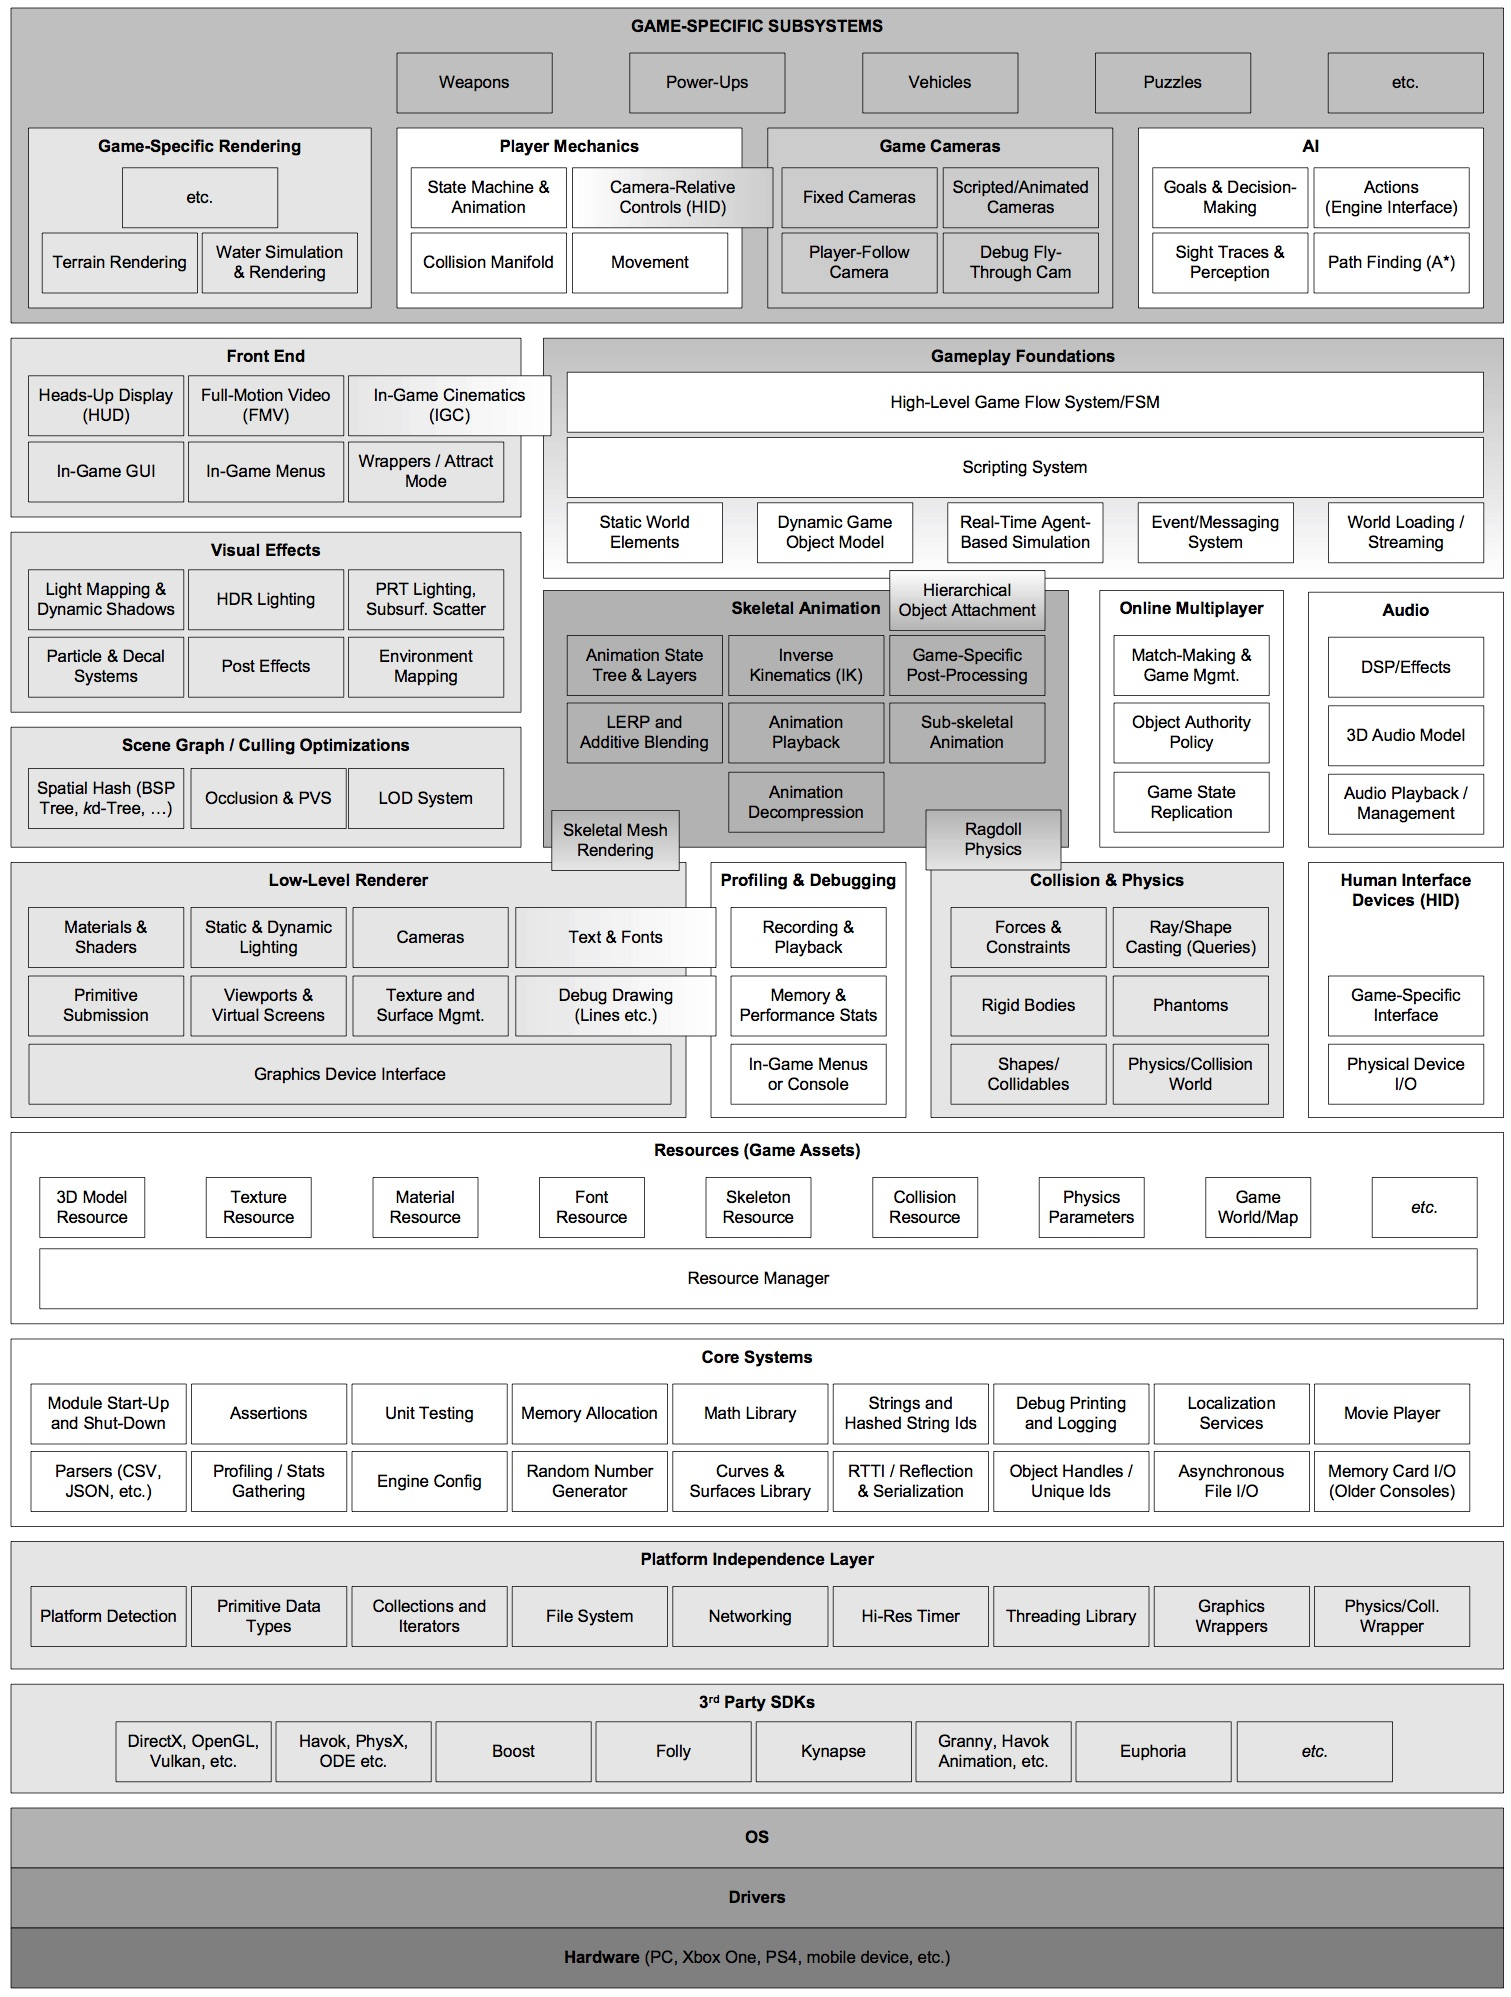
\includegraphics[center, width=0.25\textwidth]{chapter-front/pic/fig-runtime-arch.jpeg}
\caption{引擎架构图 \protect\footnotemark}
\end{figure}
\footnotetext{\nolinkurl{https://www.gameenginebook.com/figures.html}}




    \mainmatter

    \maketitle
    \part{基础知识}

    \maketitle
    \chapter{从零开始}
    \section{第一个简单项目}
作为笔记的第一部分,本节主要介绍从零开始搭建一个小型项目的过程。
大部分的C++项目都需要选择一个基本的编译配置,而CMake是其中一个流行的选择。
从github看去,很多国内外大型的开源项目都选择了CMake进行项目的配置和管理。前几年我也是CMake的推荐者,
但学习过CMake的我仍然觉得CMake过于死板,需要学习额外的DSL(Domain Specific Language),学习曲线比较陡峭。
经过查找,我发现了一个国产的开源项目xmake\footnote{\nolinkurl{https://xmake.io}},可以用Lua编写项目配置文件,符合C++编译过程的直觉,且可以通过xmake避免复杂繁琐的外部库安装配置过程,让人感觉很舒心。
最终本项目决定使用xmake作为项目配置软件。\\

当然,本项目从熟悉的Hello World开始,一步步搭建起项目框架。首先是函数主体:\\

\lstinputlisting[
    style=C++,title={main.cpp} \label{chapter-start/code/main.cpp}
]{chapter-start/code/main.cpp}

这个就是简单的标准的Hello World,通过xmake可以简单的配置项目:\\

\lstinputlisting[
    style=Lua,title={xmake.lua} \label{chapter-start/code/xmake.lua}
]{chapter-start/code/xmake.lua}

在命令行输入\emph{xmake}后,就可以自动编译项目,输入\emph{xmake r hello\_world}后,就可以运行对应项目。
通过这种流程,可以进行快速的项目编译与运行测试。\\

在后续章节中,若是对应的模块代码过于冗长,我将使用伪代码的形式提供运行的主要流程,对于的代码可以在github仓库中查看。

    \section{内存检测模块}

作为第一个编写的模块,我选择了内存检测的模块。该模块的目的是提供一个跨平台,线程安全的内存泄漏检测器。
参考了Vorbrodt的Blog\footnote{\nolinkurl{https://vorbrodt.blog/2021/05/27/how-to-detect-memory-leaks/}},
对其添加了线程安全锁后,实现了一个小型的内存检测器。
由于通过宏定义完成了内存检测器的行数输出,所以该检测器只能用于普通的new和delete,
对于placement new就无力处理了。若想要不用宏定义也可以获取代码调用位置,
可能就只能等待C++20的std::source\_location的功能了。

该内存检测模块主要通过检测new与delete的配对问题来检测内存泄漏。
一次new对应一次delete,一次new[]对应delete[],避免错配。
该模块使用了set来存储信息,在new的过程中插入信息,delete的过程中检测并删除对应new的信息,达到匹配的效果。
为了能够在程序退出时自动输出内存泄漏检查信息,定义了一个{\itshape dump\_all}的全局变量,
当程序退出时,该变量自动析构,执行最后的内存泄漏检测并输出结果。

\lstinputlisting[
    style=C++,title={MemoryCheck.h} \label{chapter-start/code/MemoryCheck.h}
]{chapter-start/code/MemoryCheck.h}

\lstinputlisting[
    style=C++,title={MemoryCheck.cpp} \label{chapter-start/code/MemoryCheck.cpp}
]{chapter-start/code/MemoryCheck.cpp}

关于内存检测模块,后续仍有很多改进空间,首先需要的就是移除宏定义对new和delete的限制,
使其能够运行调用placement的new与delete版本,以及可以在此添加自定义的内存管理器,进行自定义内存分配策略。
在新的C++中,已经有内存管理器的相关内容,在未来的看法中,可以考虑基于C++标准库来实现内存管理的功能。

除此之外,还可以通过重载new与delete函数,来调用别的底层内存分配库,比如在这里利用了微软推出的mi\_malloc库,相比系统自带的malloc函数,可以提供更高的性能。
不过需要注意的是,在不同的模块间,若采用了不同的底层内存库,有可能导致程序运行时出差,难以排查,这点需要额外注意。

\lstinputlisting[
    style=C++,title={MemoryDefine.h} \label{chapter-start/code/MemoryDefine.h}
]{chapter-start/code/MemoryDefine.h}

\lstinputlisting[
    style=C++,title={MemoryDefine.cpp} \label{chapter-start/code/MemoryDefine.cpp}
]{chapter-start/code/MemoryDefine.cpp}

% \begin{breakablealgorithm}
% \caption{Init Records} \label{initialize function}
% \begin{algorithmic}
%     \Procedure{Init Records}{$size$}
%         \State Initialize Static \emph{MemoryRecord Set}
%         \State Initialize Static \emph{DeleteTypeMismatch List}
%         \State Initialize Static \emph{MultiDelete List}
% \EndProcedure
% \end{algorithmic}
% \end{breakablealgorithm}

% \begin{breakablealgorithm}
% \caption{New} \label{new function}
% \begin{algorithmic}
% \Procedure{new}{$size$}                  \Comment{new function}
%     \State malloc a Memory Block
%     \State Insert a Memory Block Info in \emph{MemoryRecord Set}
%     \State return Memory Block Pointer
% \EndProcedure
% \end{algorithmic}
% \end{breakablealgorithm}

% \begin{breakablealgorithm}
% \caption{Delete} \label{delete function}
% \begin{algorithmic}                     \Comment{delete function}
% \Procedure{delete}{$ptr$}
%     \State result = Find $ptr$ in \emph{Memory Record Set}
%     \If{$result = True$}
%         \If{$delete type match$}
%             \State Remove Pointer Info in \emph{MemoryRecord Set}
%         \Else
%             \State Record Info in \emph{DeleteTypeMismatch List}
%         \EndIf
%     \Else
%         \State Record Info in \emph{MultiDelete List}
%     \EndIf
% \EndProcedure
% \end{algorithmic}
% \end{breakablealgorithm}

% \begin{breakablealgorithm}
% \caption{ExitCheck} \label{exit check}
% \begin{algorithmic}
% \Procedure{ExitCheck}{$ptr$}
%         \State Find Leak in \emph{MemoryRecord Set} and Dump Info
%         \State Find Mismatch in \emph{DeleteTypeMismatch List} and Dump Info
%         \State Find Mismatch in \emph{MultiDelete List} and Dump Info
% \EndProcedure
% \end{algorithmic}
% \end{breakablealgorithm}

    \section{打开第一个窗口}
当然作为一个3D程序,需要通过显示器才能展示我们的工作成果。不同的系统有不同的显示API,为了保证本项目的跨平台能力,
需要尽可能一致的为不同平台提供相同的封装,在这里本项目选择了常用的GLFW库\footnote{\nolinkurl{https://www.glfw.org/}}。\\

本项目有两套渲染器,一个是Vulkan渲染器,一个是软渲染器。软渲染器在CPU中渲染完图片后,使用OpenGL进行屏幕渲染输出,
该软渲染器主要参考了GAMES102课程的代码\footnote{\nolinkurl{https://games-cn.org/games102/}}。
根据LearnOpenGL教程\footnote{\nolinkurl{https://learnopengl-cn.github.io/}},可以很容易写出第一个窗口程序:\\

\lstinputlisting[
    style=C++,title={glfw.cpp} \label{chapter-start/code/glfw.cpp}
]{chapter-start/code/glfw.cpp}

之后开展的渲染学习项目,将从这段程序开始扩展,并接入软渲染器来实现场景初步渲染的能力。

    \section{日志输出}

\subsection{为什么需要日志输出}
在程序运行过程中,除了编译器带给我们的单步调试功能,开发过程中也需要额外的信息输出方式,
用于快速检查程序输出内容是否正常以及快速定位可能存在bug的代码位置。
比如输出log日志可以快速检测各个模块初始化是否按照预定顺序执行,是否全部成功初始化;
在调用函数的过程中,可以检测运行逻辑是否与预期一样。
更重要的是,在发布出去的软件中,我们对其进行错误追踪的方式可能只有日志输出一个渠道,
所以有一个完善的日志输出模块,对我们的开发工作会有很大帮助。
为了达到这个目的,本节主要介绍日志输出的部分。

\subsection{封装日志模块}
日志输出模块首先需要保证系统性能,其次可以按照不同的日志等级输出信息,便于分类,再次则需要保证多线程输出信息的安全,
最后则是能够输出到日志文件等功能。经过挑选,本项目采用了spdlog作为日志输出的底层库,并对其进行了简单的封装。
主要包括$Log.h^{\ref{chapter-start/code/Log.h}}$与$Log.cpp^{\ref{chapter-start/code/Log.cpp}}$两个文件。
在程序运行开始需要初始化Log,在项目终止时需要终止日志输出(虽然可以依靠自动析构,但是显式调用可以使流程更加清晰)。
利用宏定义,可以快速添加新的日志分类。

\lstinputlisting[
    style=C++,title={Log.h} \label{chapter-start/code/Log.h}
]{chapter-start/code/Log.h}

\lstinputlisting[
    style=C++,title={Log.h} \label{chapter-start/code/Log.cpp}
]{chapter-start/code/Log.cpp}

    \section{模块接口}

为了更加明确各个部分的功能,这个小节主要描述模块通用的接口,
不同的功能根据具体模块进行扩展。在此引入了IRuntimeModule这个基类,所有的模块均继承自这个类,保证了各个模块接口的统一。

\lstinputlisting[
    style=C++,title={IRuntimeModule.h} \label{chapter-start/code/IRuntimeModule.h}
]{chapter-start/code/IRuntimeModule.h}

模块运行的流程如下所示:

\begin{breakablealgorithm}
\caption{Main Loop}
\label{mainloop function}
\begin{algorithmic}
\Procedure{Main Loop}{}
    \State Init Modules
    \State Init Timer
    \While{$isRunning$}
        \State Update Timer
        \State Tick Module
    \EndWhile
    \State Finalize Modules
\EndProcedure
\end{algorithmic}
\end{breakablealgorithm}


    \maketitle
    \chapter{基本算法}
    本章主要介绍一些可能用在引擎中的基本数据结构及基本算法,包括排序和查找算法。
本书的算法主要参考算法第四版\footnote{\nolinkurl{https://algs4.cs.princeton.edu/home/}},
所以很多算法和数据结构的设计会比较类似Java的代码。
虽然本章会介绍很多数据结构与算法,但是在实际应用中,还是考虑尽量使用标准库来完成对应的功能,以提高代码通用性与可读性,方便移植到新的平台。


    % \section{算法分支-基本数据结构}

本节主要介绍一些常用的基本数据结构,包括基于数组与基于链表的,
这些数据结构共同构成后续算法部分的基石。
本节所描述的数据结构不保证多线程安全,若需要多线程,则需要后续的修改。

\subsection{Bag}

Bag指的是只能添加不能取出,所有数据的排列按照放入数据的顺序进行。

    % \section{算法分支-排序算法}

    % \section{算法分支-查找算法}


    \maketitle
    \chapter{设计模式}
    设计模式主要针对已经存在的问题,抽象解决方法。


    \maketitle
    \chapter{计算机硬件相关}
    为了深入了解计算机的运行原理,加深对程序编译与运行流程的的理解,
本章主要介绍构造LC3 Computer\footnote{\nolinkurl{https://en.wikipedia.org/wiki/Little_Computer_3}}的虚拟机,
并构建一个相对简单的C程序编译器,来生成LC3运行的汇编代码,最后通过汇编代码生成二进制文件,在虚拟机中运行。
这个虚拟机可以运行运行比较简单的程序,也可以别人编写的2048小程序\footnote{\nolinkurl{https://github.com/rpendleton/lc3-2048}}。

使用LC3作为计算机原理展示的例子,不仅仅是因为这个出现在了Introduction to Computing Systems: From Bits and Gates to C and Beyond, 2nd Edition\footnote{\nolinkurl{https://highered.mheducation.com/sites/0072467509/index.html}}一书中,
也因为这个系统结构简单,且其运行的指令集与当前电脑运行的指令集有很多相似的地方,可以由此抛砖引玉,沿着这个方向继续深入学习。

本章的内容主要参考以下几个资料\footnote{\nolinkurl{https://justinmeiners.github.io/lc3-vm/}}。

    \section{LC3电脑结构简介}

LC3的电脑结构\footnote{\nolinkurl{http://users.ece.utexas.edu/~patt/07s.360N/handouts/360n.appC.pdf}}较为简单,
它的指令集模仿了x86的指令集,是一个精简版的指令集,但是这个LC3电脑拥有现代CPU的所有基本概念,非常适合用于初学者学习研究。

LC3的最大内存为65536个uint16\_t,它的最大内存空间为128KiB,虽然很小,但是足够运行一些示例程序。
当然,作为一个虚拟机,该内存空间也可以扩展,加载更大与更复杂的程序。在虚拟机中,内存使用uint16\_t的数组来表示。

在LC3中,它的CPU通过寄存器来操作数据,执行指定指令。LC3一共有10个寄存器,分别是R0-R7一共8个通用寄存器,一个PC指令寄存器和一个COND标志位寄存器。
通用寄存器可以进行各种程序计算,PC寄存器指向下一个待执行的指令,COND寄存器保存之前计算的结果标志。寄存器在虚拟机中同样由数组表示。

\subsection{LC3指令集}

指令用于告诉CPU应该执行什么样的操作,以及该操作附带的参数。
在LC3中仅有16个指令,每个指令16bit长,左4位用于表示指令代码,其余位数用于存储指令参数。
这16个指令分别为:OP\_BR、OP\_ADD、OP\_LD、OP\_ST、OP\_JSR、OP\_AND、OP\_LDR、OP\_STR、OP\_RTI、OP\_NOT、OP\_LDI、OP\_STI、OP\_JMP、OP\_RES、OP\_LEA、OP\_TRAP。
由于LC3的指令数量很少,该指令集属于RISC指令集\footnote{\nolinkurl{https://en.wikipedia.org/wiki/Reduced_instruction_set_computer}}。

\subsection{标志位}

LC3的标志位仅有三个符号:FL\_POS、FL\_ZRO、FL\_NEG。该符号用于表示逻辑表达式的比较结果。

    \section{虚拟机实现}

虚拟机的执行主要分为以下几步:

1.从PC寄存器加载指令

2.对PC寄存器加一

3.根据加载的指令决定执行命令

4.执行命令

5.回到第一步

指令的执行在虚拟机里使用switch case来决定执行程序。这个虚拟机的运行流程十分简单,具体实现代码如下:

% \lstinputlisting[
%     style=C++,title={lc3vm.h} \label{chapter-hardware/code/lc3vm.h}
% ]{chapter-hardware/code/lc3vm.h}

% \lstinputlisting[
%     style=C++,title={lc3vm.c} \label{chapter-hardware/code/lc3vm.c}
% ]{chapter-hardware/code/lc3vm.c}

% \lstinputlisting[
%     style=C++,title={lc3.c} \label{chapter-hardware/code/lc3.c}
% ]{chapter-hardware/code/lc3.c}

\lstinputlisting[
    style=C++,title={lc3.c} \label{chapter-hardware/code/lc3vm-other.c}
]{chapter-hardware/code/lc3vm-other.c}

这个虚拟机还有高级版本,可以加载一个微型的系统,代替c的switch case


    \maketitle
    \part{基础模块}

    \maketitle
    \chapter{文件系统}
    本章主要介绍我自己设计的一套文件系统,该系统的主要功能是方便用户使用统一的方式加载资源文件,不论资源文件的存储位置,是否进行压缩。
在统一文件加载方式后,我们在开发过程中,可以直接进行系统目录下的文件操作,并方便的对其进行修改。
而当项目完成并将资源打包后,程序也可以利用同一套API直接进行打包的资源文件的操作,不需要额外的修改代码,方便了开发、调试与发布。
    \section{文件管理系统简介}


    \maketitle
    \chapter{资源管理}
    \input{chapter-resource/chapter-resource-00.tex}

    \maketitle
    \chapter{内存管理}
    \input{chapter-memory/chapter-memory-00.tex}

    \maketitle
    \chapter{多线程相关}

    \maketitle
    \chapter{程序中的数学}
    \input{chapter-math/chapter-math-00.tex}

    \maketitle
    \part{中级模块}

    \maketitle
    \chapter{渲染}

    \maketitle
    \chapter{物理}

    \maketitle
    \chapter{脚本系统}

    \appendix
    \maketitle
    \chapter{附录}

    % \maketitle
    % \chapter{参考文献}
    % %[1] һ�ݣ���̫����̵�LATEX2�� ����. https://mirrors.tuna.tsinghua.edu.cn/CTAN/info/lshort/chinese/lshort-zh-cn.pdf \\
%[2] Game Engine Architecture 3rd. https://www.gameenginebook.com/index.html \\
%[3] 


    \backmatter
    \chapter{后记}

    %\bibliography{books} % 利用 BibTeX 工具从数据库文件 books.bib 生成参考文献
    %\printindex % 利用 makeindex 工具生成索引

\end{document}
% Local Variables:
% TeX-engine: xetex
% End:
